%\title{beavtex}
\documentclass[double, 1.5in, 12pt]{beavtex}
\usepackage{graphicx}
\usepackage{rotating} %Package added to allow the rotation of figures and chart on a page, {sidewaysfigure} command
\usepackage{tablefootnote} %Packaged added to allow footnotes in the tabular environment, use \tablefootnote command
\usepackage{amsmath}
\usepackage{amsfonts}
\usepackage{color}
 \usepackage[ruled,vlined,linesnumbered,resetcount,algochapter]{algorithm2e}

\title{Trabajo Pr\'actico N\'umero 1:}
\subtitle{"No creo que a \'el le gustara eso"}
\Agustina{Aldasoro, Agustina \ agusaldasoro@gmail.com}
\Belen{Bouz\'on, Mar\'ia Bel\'en \ belenbouzon@gmail.com}
\Gustavo{Cairo, Gustavo Juan \ gjcairo@gmail.com}

\submitdate{4 de Septiembre de 2014}


\usepackage{todonotes}

\newcommand{\real}{\mathbb{R}}
\newcommand{\nat}{\mathbb{N}}

\newcommand{\atacante}{sanguijuela}
\newcommand{\capitan}{Capit\'an Guybrush Threepwood}
\newcommand{\objeto}{parabrisas}
\newcommand{\nave}{El Pepino Marino}

\newcommand{\revJ}[1]{{\color{red} #1}}



\begin{document}
\maketitle
\mainmatter

%-------------------------INTRODUCTION-----------------------------

\chapter{Introducci\'on Te\'orica}

Hab\'iendonos sido proporcionados:

\begin{itemize}
\item la ecuaci\'on del calor que modela de forma gen\'erica el comportamiento de la temperatura T en un punto (x,y) $\in$ $\mathbb{R}^2$ luego de haber consolidado un estado estacionario (figura 1.1) \\

\begin{equation}
\frac{\partial^2T(x,y)}{\partial x^{2}}+\frac{\partial^2 T(x,y)}{\partial y^{2}} = 0.
\end{equation}

\item las medidas de un hipot\'etico parabrisas bidimensional cuyos m\'argenes se sabe que mantendr\'an una temperatura constante de -100ºC 

\item y ciertas posiciones del mismo que ser\'an sometidas a una temperatura constante (tambi\'en conocida) aplicada por  una clase id\'ilica y mutante de filo an\'elidos llamados hirud\'ineos (com\'unmente conocidos como "sanguijuelas"),

\end{itemize}

nuestros desaf\'ios consisten en:

\begin{itemize}

\item Proveer un algoritmo que - a partir de la consideraci\'on de los datos reci\'en citados - aproxime la temperatura esperada en condiciones de estabilidad en una cantidad finita de puntos del parabrisas. 

\item Optimizar dicho algoritmo aprovechando los beneficios potencialmente provistos por la estructura del sistema de ecuaciones planteado.

\item Dise\~nar e implementar una funci\'on algor\'itmica que garantice, a partir de la eliminaci\'on de la menor cantidad posible de sanguijuelas, la perdurabilidad del parabrisas (esto es, el resguardo de su punto cr\'itico a una temperatura inferior a los 235 grados Celcius).

\end{itemize}

Como punto de partida y linea de desarrollo que nos permita conseguir estos objetivos, haremos uso e implementaremos en C++ el Algoritmo de Eliminaci\'on Gaussiana, poniendo en discusi\'on posteriormente posibles modificaciones del mismo que permitan adecuarlo a diversos contextos y necesidades.

Dicho algoritmo transforma un sistema lineal Ax= b, A $\in \mathbb{R}^{nxn}$, en uno equi- \- valente Ux=y - donde U es una matriz triangular superior - permitiendo aplicar posteriormente el algoritmo de sustituci\'on regresiva que culmina en la resoluci\'on total del sistema.







%------------------------DESARROLLO--------------------------------

%\chapter{Desarrollo}

\section{Planteo del Sistema de Ecuaciones}

Al  comenzar a plantear un sistema de ecuaciones que pudiera resultar efectivo para la resoluci\'on de los problemas presentados, se puso en cuesti\'on inicialmente el que se desarrolla a continuaci\'on:

Considerando la ecuaci\'on de aproximaci\'on por diferencias finitas de la ecuaci\'on del calor
\begin{equation}
t_{ij} \ =\ \frac{ t_{i-1,j} + t_{i+1,j} + t_{i,j-1} + t_{i,j+1}}{4}.\label{eq:calordd}
\end{equation}
pensamos que podr\'iamos diseñar una matriz que tuviera para todo i,j una ecuaci\'on asociada en funci\'on de las otras posiciones y que estuviera extendida con cada valor de $t_{ij}$ en el vector independiente (es decir, un sistema de ecuaciones expresadas como en la figura 2.1). R\'apidamente descartamos esa posibilidad, ya que nos encontr\'abamos situando en el vector de t\'erminos independientes, varios que eran ciertamente dependientes.

Luego volvimos a la ecuaci\'on de la que hab\'iamos partido, que nos indicaba la propiedad que inexorablemente cumpl\'ia el comportamiento de la temperatura en funci\'on de la posici\'on consultada  y de la distribuci\'on de las sanguijuelas.  Le restamos a ambos lados $t_{ij}$ y, despejando la ecuaci\'on, obtuvimos una nueva expresi\'on igualada a cero, que determinar\'a finalmente la estructura de nuestro sistema de ecuaciones, dado por:

\begin{equation}
0 \ =\  t_{i-1,j} + t_{i+1,j} + t_{i,j-1} + t_{i,j+1} - 4.t_{i,j+1}\label{eq:calordd}
\end{equation}

para todos aquellos puntos a los que no se les aplica una temperatura constante  (es decir, no pertenecen al borde del parabrisas ni se encuentran ocupados por sanguijuelas).

	$T_{ij}$=-100 para todos los puntos del borde.

	$T_{ij}$= $T_s$ para los puntos ocupados por sanguijuelas, siendo $T_s$ la temperatura aplicada por las sanguijuelas.


\section{Planteo acerca de las estructura internas de las matrices}

Para representar matrices consideramos inicialmente la estructura cl\'asica: $vector<vector<double>>$. \\
Esta implementaci\'on permite acceder al elemento M$_{ij}$ mediante la sentencia $matriz[i][j]$. \\
Almacenamos cada punto discretizado del parabrisas como una inc\'ognita de la matriz, es decir si tenemos una discretizaci\'on de $n+1$ filas por $m+1$ columnas, tendremos una matriz de $(n+1).(m+1)$ filas y $(n+1).(m+1)$ columnas. Si quiero acceder al elemento de la fila $i$, columna $j$ del parabrisas discretizado: considero la inc\'ognita de la columna de la matriz $(k.i)+ j$, siendo $k=\frac{a}{h}+1$. \\
En cuanto al almacenamiento de nuestra matriz banda, al considerar su morfolog\'ia nos pareci\'o una idea plausible representarla conservando  \'unicamente, los elementos no nulos de la bandas, de la diagonal principal y los t\'erminos independientes. Vi\'endolo gr\'aficamente, si la matriz fuera la siguiente:


$
\left(
       \begin{array}{p{5mm}p{5mm}p{5mm}p{5mm}p{5mm}p{5mm}p{5mm}p{5mm}p{5mm}p{5mm}}
1 & 0 & 0 & 0 & 0 & 0 & 0 & 0 & 0 & 0 \\
0 & 1 & 0 & 0 & 0 & 0 & 0 & 0 & 0 & 0 \\
0 & 0 & 1 & 0 & 0 & 0 & 0 & 0 & 0 & 0 \\
0 & 0 & 0 & 1 & 0 & 0 & 0 & 0 & 0 & 0\\
1 & 0 & 0 & 1 & -4 & 1 & 0 & 0 & 1 & 0 \\
0 & 1 & 0 & 0 & 1 & -4 & 1 & 0 & 0 & 1 \\
0 & 0 & 0 & 0 & 0 & 0 & 1 & 0 & 0 & 0\\
0 & 0 & 0 & 0 & 0 & 0 & 0 & 1 & 0 & 0\\
0 & 0 & 0 & 0 & 0 & 0 & 0 & 0 & 1 & 0\\
0 & 0 & 0 & 0 & 0 & 0 & 0 & 0 & 0 & 1\\

       \end{array}
\right)
$
\emptyline
\emptyline
\emptyline
Se almacenar\'ia de esta forma:\\

$
\left(
       \begin{array}{p{5mm}p{5mm}p{5mm}p{5mm}p{5mm}}
0 & 0 & 1 & 0 & 0\\
0 & 0 & 1 & 0 & 0\\
0 & 0 & 1 & 0 & 0\\
0 & 0 & 1 & 0 & 0\\
 1 & 1 & -4 & 1 & 1 \\
 1 & 1 & -4 & 1 & 1 \\
0 & 0 & 1 & 0 & 0\\
0 & 0 & 1 & 0 & 0\\
0 & 0 & 1 & 0 & 0\\
0 & 0 & 1 & 0 & 0\\
       \end{array}
\right)
$


\[
 \begin{array}{p{6mm}p{6mm}p{6mm}p{6mm}p{6mm}p{6mm}}

\end{array}
\]


Posteriormente advertimos que aquella estructura podr\'ia traernos serios inconvenientes al momento de utilizarla como par\'ametro en el algoritmo de eliminaci\'on gaussiana e intentar hallar la soluci\'on al sistema, dado que los ceros que se encuentran a la derecha de la diagonal y a la izquierda son potencialmente modificables durante este procedimiento, y dichos cambios ser\'ian imperceptibles a pesar de ser determinantes a la hora de hallar la soluci\'on del sistema.

Ejemplo: 

Consideremos la siguiente matriz M $\in \mathbb{R}^{16x17}$ producida a partir de un parabrisas cuadrado de 3 metros de lado, sin sanguijuelas, discretizado definiendo arbitrariamente h=1.

$
\left(
       \begin{array}{p{5mm}p{5mm}p{5mm}p{5mm}p{5mm}p{5mm}p{5mm}p{5mm}p{5mm}p{5mm}p{5mm}p{5mm}p{5mm}p{5mm}p{5mm}p{5mm}|c}
 1 & 0 & 0 & 0 & 0 & 0 & 0 & 0  & 0 & 0 & 0 & 0 & 0 & 0 & 0 & 0 & -100  \\
 0 & 1 & 0 & 0 & 0 & 0 & 0 & 0  & 0 & 0 & 0 & 0 & 0 & 0 & 0 & 0 & -100  \\
 0 & 0 & 1 & 0 & 0 & 0 & 0 & 0  & 0 & 0 & 0 & 0 & 0 & 0 & 0 & 0 & -100  \\
 0 & 0 & 0 & 1 & 0 & 0 & 0 & 0  & 0 & 0 & 0 & 0 & 0 & 0 & 0 & 0 & -100  \\
 0 & 0 & 0 & 0 & 1 & 0 & 0 & 0  & 0 & 0 & 0 & 0 & 0 & 0 & 0 & 0 & -100  \\
 0 & 1 & 0 & 0 & 1 & -4 & 1 & 0  & 0 & 1 & 0 & 0 & 0 & 0 & 0 & 0 & 0  \\
 0 & 0 & 1 & 0 & 0 & 1 & -4 & 1  & 0 & 0 & 1 & 0 & 0 & 0 & 0 & 0 & 0  \\
 0 & 0 & 0 & 0 & 0 & 0 & 0 & 1  & 0 & 0 & 0 & 0 & 0 & 0 & 0 & 0 & -100  \\
 0 & 0 & 0 & 0 & 0 & 0 & 0 & 0  & 1 & 0 & 0 & 0 & 0 & 0 & 0 & 0 & -100  \\
 0 & 0 & 0 & 0 & 0 & 1 &  0 & 0  & 1 & -4 & 1 & 0 & 0 & 1 & 0 & 0 & 0  \\
 0 & 0 & 0 & 0 & 0 & 0 & 1 & 0  & 0 & 1 & -4 & 1 & 0 & 0 & 1 & 0 & 0  \\
 0 & 0 & 0 & 0 & 0 & 0 & 0 & 0  & 0 & 0 & 0 & 1 & 0 & 0 & 0 & 0 & -100  \\
 0 & 0 & 0 & 0 & 0 & 0 & 0 & 0  & 0 & 0 & 0 & 0 & 1 & 0 & 0 & 0 & -100  \\
 0 & 0 & 0 & 0 & 0 & 0 & 0 & 0  & 0 & 0 & 0 & 0 & 0 & 1 & 0 & 0 & -100  \\
 0 & 0 & 0 & 0 & 0 & 0 & 0 & 0  & 0 & 0 & 0 & 0 & 0 & 0 & 1 & 0 & -100  \\
 0 & 0 & 0 & 0 & 0 & 0 & 0 & 0  & 0 & 0 & 0 & 0 & 0 & 0 & 0 & 1 & -100  \\
       \end{array}
\right)
$

\emptyline
En este caso, si la Eliminaci\'on Gaussiana se estuviera encargando de anular los valores que se encuentran por debajo de la diagonal principal en la quinta columna, eventualmente el resultado en la novena fila ser\'a, para todo j / $ 0<=j<=15$  \begin{equation}
(a'_{9,j}) = (a_{9,j}) - 4^{-1}*(a_{5,j})
\end{equation}

Es decir que el elemento $a'_{9,6}$ deber\'a pasar a valer $-4^{-1}$ , pero a causa de un error en la estructura de representaci\'on estr\'iamos omitiendo la relevancia de su modificaci\'on y arribando, en consecuencia, a un resultado incorrecto.

Teniendo en cuenta este inconveniente, resolvimos escoger una opci\'on similar que a nivel espacial era peor que la reci\'en mencionada pero segu\'ia aventajando a la opci\'on cl\'asica. Esta tercera alternativa consisti\'o en computar para cada fila de la matriz original s\'olo los elementos que se encontraran entre el extremo izquierdo de la banda y el derecho (inclusive).
La matriz presentada con anterioridad quedar\'ia almacenada de la siguiente manera:\\

$
\left(
       \begin{array}{p{5mm}p{5mm}p{5mm}p{5mm}p{5mm}p{5mm}p{5mm}p{5mm}p{5mm}p{5mm}}
 0 & 0 & 0 & 0 & 1 & 0 & 0 & 0 & 0\\
 0 & 0 & 0 & 0 & 1 & 0 & 0 & 0 & 0\\
 0 & 0 & 0 & 0 & 1 & 0 & 0 & 0 & 0\\
 0 & 0 & 0 & 0 & 1 & 0 & 0 & 0 & 0\\
1 & 0 & 0 & 1 & -4 & 1 & 0 & 0 & 1 \\
1 & 0 & 0 & 1 & -4 & 1 & 0 & 0 & 1 \\
 0 & 0 & 0 & 0 & 1 & 0 & 0 & 0 & 0\\
 0 & 0 & 0 & 0 & 1 & 0 & 0 & 0 & 0\\
 0 & 0 & 0 & 0 & 1 & 0 & 0 & 0 & 0\\
 0 & 0 & 0 & 0 & 1 & 0 & 0 & 0 & 0\\
       \end{array}
\right)
$




\[
 \begin{array}{p{6mm}p{6mm}p{6mm}p{6mm}p{6mm}p{6mm}p{6mm}p{6mm}p{6mm}p{6mm}}

\end{array}
\]

Este modo junto con el cl\'asico fueron los que decidimos implementar para experimentar y contrastar sus comportamientos en relaci\'on a los algoritmos que desarrollar\'iamos.

\section{Planteo en relaci\'on al empleo de nuestras estructuras en el problema presentado}


Al momento de recibir por par\'ametro las coordenadas del centro de cada sanguijuela, nuestra matriz de posiciones deb\'ia adaptar sus valores de acuerdo al mapeo que se har\'ia de cada una de ellas en el nuevo modelo discreto de representaci\'on. En funci\'on de la longitud de su radio, la ubicaci\'on de su centro y la medida de discretizaci\'on escogida, los mencionados espec\'imenes podr\'ian pasar a estar representados en un \'unico punto, en varios o incluso en ninguno. 
En principio, para cada sanguijuela deb\'iamos recorrer posici\'on a posici\'on de la matriz discretizada averiguando si pertenec\'ia al sector abarcado por la misma. Para evitarlo, calculamos previamente, a partir de los par\'ametros, un sector cuadrado de puntos fuera de los cuales no existir\'ia la posibilidad de que una sanguijuela en particular tuviera injerencia directa. Determinado este sector, s\'olo deber\'iamos modificar los puntos $p$ pertenecientes al mismo que cumplieran, a su vez,
 
\begin{equation}
\sqrt{{(p1-c1)}^2 + {(p2-c2)}^2}  \leq  radio
\end{equation}

Esto lo cumplen aquellos puntos discretizados que representan a alguna coordenada del cont\'inuo cuya distancia al centro C=(c1,c2) de la sanguijuela  es menor o igual al radio de la misma. A dichas posiciones se les asignar\'a posteriormente la temperatura T$_s$ en la matriz de temperaturas, mientras que a las restantes les corresponder\'a la ecuaci\'on de la figura 1.1.

Teniendo en cuenta el empleo subyacente de la aritm\'etica finita, consideramos que planteando una ecuaci\'on equivalente elevando al cuadrado a ambos lados de la desigualdad - eliminando el c\'alculo de la ra\'iz cuadrada - podr\'iamos lograr una mayor precisi\'on y una menor probabilidad de error. Por ende, la ecuaci\'on (2.4) fue sustitu\'ida por la siguiente:

\begin{equation}
{(p1-c1)}^2 + {(p2-c2)}^2  \leq  {radio}^2
\end{equation}

En relaci\'on a los casos en que al pasar del plano cont\'inuo al discreto la presencia de las sanguijuelas no se ve\'ia reflejada en ning\'un punto, nos pareci\'o una buena pr\'actica pensar alg\'un criterio para diferenciar y advertir al usuario sobre aquellas discretizaciones que se pudieran considerar como "buenas" de otras que pudieran favorecer la aparici\'on de casos patol\'ogicos en los cuales el c\'alculo de la estimaci\'on de la temperatura fuera groseramente inexacto. Algunos de estos casos se mencionan a continuaci\'on: \\
\emptyline
\textit{-La sanguijuela no tiene ning\'un punto discretizado en su interior.} \\
A fines de preservar el parabrisa, si esto ocurre en puntos cerca del borde no nos es de mayor inter\'es. En cambio, si la ubicaci\'on de la sanguijuela es cerca del punto cr\'itico podr\'ia influir notablemente en su temperatura. Cabe recalcar, que hay que tener en cuenta que esto var\'ia de acuerdo al radio y la temperatura de las sanguijuelas. \\
\emptyline
\textit{-La cantidad de sanguijuelas que no tiene ning\'un punto discretizado en su interior y est\'an cerca del punto cr\'itico es alta.} \\
Podr\'ia pasar que haya una cantidad "alta" de sanguijuelas cerca del borde, pero ninguna tenga un punto en su interior que este discretizado. Las sanguijuelas est\'an, s\'olo que nuestra discretizaci\'on no les permite influir en la temperatura del punto central.\\
\emptyline
\textit{-Existe una sanguijuela que no tiene ning\'un punto discretizado en su interior, pero el punto cr\'itico si pertenece a \'el.} \\
Ejemplo: Hay una sola sanguijuela, que dado por su radio y por su centro, tiene en su interior al punto cr\'itico. En teor\'ia, el punto cr\'itico tendr\'ia el valor T$_s$, pero una vez m\'as la discretizaci\'on dada por el h no nos permitir\'ia verlo. \\
\\
ACLARACI\'ON:\\
Si la temperatura T$_s$ pasada por par\'ametro es menor que 235 grados cent\'igrados, no existe siquiera la posibilidad de que el parabrisas pase a ser inestable.\\
\\

La idea de informar al usuario sobre estos casos patol\'ogicos fue descartada debido a que en el contexto del presente trabajo cobra relevancia el estudio del comportamiento de las estructuras y algoritmos diseñados en un plano te\'orico global, en detrimento del an\'alisis de los casos particulares.

Sin embargo, sin perder de vista la proyecci\'on de nuestras implementaciones en un hipot\'etico caso real, nos pareci\'o sensato idear una forma produente de estimar la temperatura en el punto cr\'itico cuando el mismo no se hallara discretizado.
Inicialmente se nos presentaron las siguientes opciones: \\
- Adjudicarle la temperatura del punto discretizado m\'as pr\'oximo.\\
- Asignarle la temperatura del promedio de los cuatro puntos discretizados m\'as cercanos.\\
- Otorgarle la temperatura del promedio de una cantidad de puntos discretizados cercanos proporcional a la cantidad total.

Decidimos resolverlo del siguiente modo:\\
- Si el punto cr\'itico est\'a discretizado, se le otorga el valor que se calcul\'o en la discretizaci\'on. \\
- Si el punto cr\'itico est\'a ubicado en el medio del cuadrante armado por la discretizaci\'on, es decir es el \'unico caso en que est\'a a la misma distancia de los cuatro puntos discretizados m\'as cercanos, se le otorga el promedio de estos cuatro valores.\\
- Si el punto cr\'itico est\'a a la misma distancia de dos puntos discretizados, se le otorga el promedio de estos dos valores.\\
- En cualquier otro caso, se le otorga al punto cr\'itico el valor del punto discretizado m\'as cercano.\\

 {\color{red}
PODEMOS PONER LOS DIBUJITOS SI NOS SOBRA TIEMPO. Just saying.\\}


\section{Planteo en relaci\'on a la implementaci\'on del Algoritmo de Eliminaci\'on Gaussiana y back substitution}


A la hora de pensar maneras de optimizar el c\'omputo de los c\'alculos vinculados a la matriz, tomamos en cuenta la posibilidad de particionarla de forma tal que quedara dividida en patrones que pudieran repetirse, de modo que los mismos pudieran ser resueltos algor\'itmicamente una \'unica vez para luego replicar su resultado en m\'as de una oportunidad. Concluimos, finalmente , que este mecanismo resultar\'ia aplicable s\'olo en casos muy espec\'ificos para los cuales no existe ning\'un indicio de que su probabilidad de ocurrencia pudiera ser significativa. 

Habiendo descartado dicha posibilidad, decidimos optar por implementar una adaptaci\'on del algoritmo de Eliminaci\'on Gaussiana que procurara aprovechar las particularidades de la morfolog\'ia de la estructura de las matrices "Banda". 
Dicho algoritmo se implement\'o de la siguiente manera:


\IncMargin{1em}
\begin{algorithm}
\SetKwData{Left}{left}\SetKwData{This}{this}\SetKwData{Up}{up}
\SetKwFunction{Union}{Union}\SetKwFunction{FindCompress}{FindCompress}
\SetKwInOut{Input}{input}\SetKwInOut{Output}{output}
\Input{Matriz}
\Output{Void}
\BlankLine
\For{$i\leftarrow (k+2)$ \KwTo $(\# filas - k)$}{
$j\leftarrow 0$ \tcp*[f]{j va a recorrer las columnas} \\
\While{$j < (posici$\'o$n$ $elemento$ $de$ $la$ $diagonal)$}{\label{forins}
$com\leftarrow (i+j-k-1)$ \tcp*[f]{\color{red}{GUS: Poner aclaraci\'on abajo.}} \\
\If{($matriz(i,j) > \varepsilon$)}{
m $\leftarrow$ matriz(i,j)/matriz(com,PosDiagonal) \\
Resta Corrida sin la columna Resultado (fila i, fila com) \\
matriz(i, PosResult) -= matriz(com, PosResult) 
}}}
\caption{EGbanda}\label{algo_disjdecomp}
\end{algorithm}\DecMargin{1em}


Teniendo en cuenta que bajo las condiciones dadas en nuestro sistema de ecuaciones, es imposible que un elemento de la diagonal principal sea nulo o quede nulo despu\'es de triangular. Decidimos omitir el paso de la Eliminaci\'on Gaussiana donde se  asegura que al momento de triangular no quede un elemento nulo en la diagonal, mediante un intercambio de filas.

Asimismo, luego de esquematizarlo, nos planteamos la posibilidad de optimizar la eficiencia del algoritmo y minimizar su error aplicando pivoteo parcial. Sin embargo, dicha implementaci\'on tendr\'ia un costo extra en complejidad temporal y no influir\'ia en nuestros resultados dado al origen de la matriz. Cre\'imos razonable, en consecuencia, no implementarlo de esa forma en esta oportunidad.\\



Una observaci\'on de may\'uscula importancia fue notar que el primer algoritmo que desarrollamos con los fines de resolver el sistema triangulado mediante E.G, generaba resultados con errores porcentualmente grandes en relaci\'on a los tolerables. Luego de un an\'alisis te\'orico del problema, nos dimos cuenta de que nos encontr\'abamos dividiendo a cada fila por el coeficiente ubicado en la diagonal para asegurarnos de que al final de la pasada por esa fila, la misma quedara como el vector can\'onico igualado a su resultado. Esto acarreaba error porque hacia menos exacta la cuenta ya que no solo se dividia al vector resultado por un coeficiente cuyo m\'odulo no se encuentra acotado inferiormente, sino que tambi\'en se repet\'ia el procedimiento con los demas coeficientes que luego habr\'ia que triangular. \\
Por lo tanto, decidimos ir triangulando por filas, es decir, despejar cada elemento desde la \'ultima fila hacia la primera, suplantando en la ecuaci\'on superior los valores obtenidos. \'Unicamente despu\'es de este procedimiento dividir\'iamos por el coeficiente principal, de modo que quede la matriz Identidad igualada a su resultado. \\




%-------------------RESULTADOS--------------------------

\chapter{Resultados}

Cito: \\

Deben incluir los resultados de los experimentos, utilizando el formato mas adecuado
para su presentacion. Deber´an especificar claramente a que experiencia corresponde
cada resultado. No se incluir´an aqu´ı corridas de maquina\\
No es aceptable incluir tablas de resultados numericos siempre que sea posible su
graficacion. 
Esto no significa que se deban mostrar los resultados exclusivamente en forma de graficos.
Se debe buscar la manera de mostrar la informacion importante en la mejor forma de visualizacion. Este hecho sera tenido en cuenta para la evaluacion de la presentacion de los informes.
Es conveniente que el proceso de experimentacion no se realice en forma independiente
de la presentacion de los resultados, de manera que los resultados parciales obtenidos en
los primeros experimentos vayan orientando la experimentacion posterior.









%------------------------DISCUSION--------------------------------

\chapter{Discusi\'on}

Cito: \\

Se incluira aqui un analisis de los resultados obtenidos en la seccion anterior (se analizara
su validez, coherencia, etc.). Deben analizarse como mınimo los items pedidos en el
enunciado. No es aceptable decir que “los resultados fueron los esperados”, sin hacer
clara referencia a la teorıa a la cual se ajustan. Ademas, se deben mencionar los resultados interesantes y los casos "patologicos" encontrados.

La seccion de discusion debe estar relacionada indefectiblemente con el desarrollo y los
resultados presentados en las secciones anteriores. No se aceptaran afirmaciones que no esten
respaldadas por los datos presentados


\pagebreak[4]

\begin{figure}
\begin{center}
	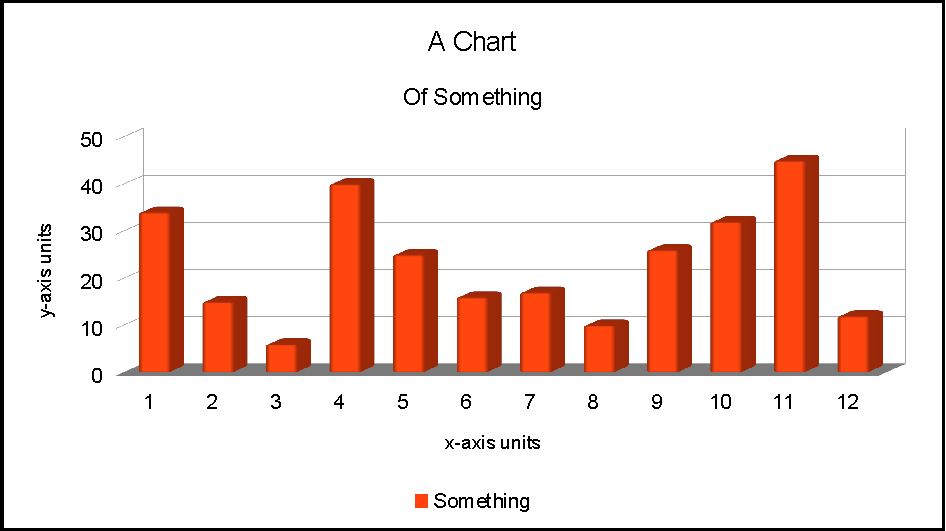
\includegraphics[width=14cm]{chart.pdf}
	\caption{A Chart.}
	\label{fig:chart}
	\end{center}
\end{figure}

\pagebreak[4]




%-----------------------CONCLUSION--------------------------------

\chapter{Conclusiones}

Cito: \\

Esta seccion debe contener las conclusiones generales del trabajo. Se deben mencionar
las relaciones de la discusion sobre las que se tiene certeza, junto con comentarios
y observaciones generales aplicables a todo el proceso. Mencionar tambien posibles
extensiones a los metodos, experimentos que hayan quedado pendientes\\
Se pide certeza y rigor logico de la discusion, el analisis y las conclusiones. Se pondra especial
enfasis en que las conclusiones se desprendan de las experiencias realizadas. 



\chapter{Ap\'endices}

\section{Ap\'endice A}


\begin{centering}
\large\bf Laboratorio de M\'etodos Num\'ericos - Segundo Cuatrimestre 2014 \\
\large\bf Trabajo Pr\'actico N\'umero 1: \emph{``No creo que a \'el le gustara eso''}\\
\end{centering}


\vskip 0.5 cm
\hrule
\vskip 0.1 cm

{\noindent \bf Introducci\'on}

El afamado \capitan\ se encuentra nuevamente en problemas. El
\objeto\ de su nave \nave\ est\'a siendo atacado simult\'aneamente por varios
dispositivos hostiles vulgarmente conocidos como \emph{\atacante s
mutantes}. Estos artefactos se adhieren a los \objeto\ de las naves y
llevan a cabo su ataque aplicando altas temperaturas sobre la superficie, con
el objetivo de debilitar la resistencia del mismo y permitir as\'\i \
un ataque m\'as mort\'\i fero. Cada \atacante\ consta de una \emph{sopapa
de ataque} circular, que se adhiere al \objeto\ y aplica una temperatura
constante sobre todos los puntos del \objeto\ en contacto con la sopapa.

Para con\-tra\-rres\-tar estas acciones hostiles, el \capitan\ 
solamente cuenta con el sistema de refrigeraci\'on de la nave, que puede
aplicar una temperatura constante de -100${}^o$C a los bordes del \objeto.
El manual del usuario de la nave dice que si el punto central del \objeto\ 
alcanza una temperatura de 235${}^o$C, el \objeto\ no resiste la temperatura
y se destruye. Llamamos a este punto el \emph{punto cr\'\i tico} del
\objeto.

En caso de que el sistema de refrigeraci\'on no sea suficiente para salvar
el punto cr\'\i tico, nues\-tro \capitan\ tiene todav\'\i a una posibilidad
adicional: puede des\-tru\-ir algunas de las \atacante s, pero debe eliminar la
menor cantidad posible de \atacante s dado que cada eliminaci\'on consume
energ\'\i a que puede ser vital para la concreci\'on de la misi\'on.
La situaci\'on es desesperante, y nuestro h\'eroe debe tomar una r\'apida
determinaci\'on: debe decidir qu\'e \atacante s eliminar de modo tal que el
\objeto\ resista hasta alcanzar la base m\'as cercana.

{\noindent \bf El modelo}

Suponemos que el \objeto\ es una placa rectangular de $a$ metros de ancho y $b$ metros de altura. Llamemos $T(x,y)$ a la temperatura en el punto dado por las coordenadas $(x,y)$. En el estado estacionario, esta temperatura satisface la ecuaci\'on del calor:

\begin{equation}\label{eq:calor}
\frac{\partial^2T(x,y)}{\partial x^{2}}+\frac{\partial^2 T(x,y)}{\partial y^{2}} = 0.
\end{equation}

\noindent La temperatura constante en los bordes queda definida por la siguiente ecuaci\'on:
\begin{equation}
T(x,y) = -100^o\textrm{C}~~~~~\textrm{si } x = 0,a \textrm{ \'o } y = 0,b.
\label{eq:borde}
\end{equation}

\noindent De forma an\'aloga es posible fijar la temperatura en aquellos puntos cubiertos por una \atacante, considerando $T_s$ a la temperatura ejercida por las mismas.

El problema en derivadas parciales dado por la primera ecuaci\'on con las condiciones de contorno presentadas recientemente, permite encontrar la funci\'on $T$ de temperatura en el \objeto, en funci\'on de los datos mencionados en esta secci\'on.

%(x_j,y_i) = (ib/n,ja/m)
Para estimar la temperatura computacionalmente, con\-si\-de\-ra\-mos la siguiente discretizaci\'on del \objeto: sea $h \in \mathbb{R}$ la granularidad de la discretizaci\'on, de forma tal que $a = m\times h$ y $b = n \times h$, con $n,m \in \mathbb{N}$, obteniendo as\'i una grilla de $(n+1)\times(m+1)$ puntos. Luego, para $i=0,1,\dots,n$ y $j=0,1,\dots,m$, llamemos $t_{ij} = T(x_j,y_i)$ al valor (desconocido) de la funci\'on $T$ en el punto $(x_j, y_i) = (ih, jh)$, donde el punto $(0,0)$ se corresponde con el extremo inferior izquierdo del \objeto.
La aproximaci\'on por \emph{diferencias finitas} de la ecuaci\'on del calor afirma que:
\begin{equation}
t_{ij} \ =\ \frac{ t_{i-1,j} + t_{i+1,j} + t_{i,j-1} + t_{i,j+1}}{4}.\label{eq:calordd}
\end{equation}

Es decir, la temperatura de cada punto de la grilla debe ser igual al promedio de las tem\-pe\-ra\-tu\-ras de sus puntos vecinos en la grilla. Adicionalmente, conocemos la temperatura en los bordes, y los datos del problema permiten conocer la temperatura en los puntos que est\'an en contacto con las \atacante s.

{\noindent \bf Enunciado}

Se debe implementar un programa en \verb+C+ o \verb-C++- que tome como entrada los par\'ametros del problema ($a$, $b$, $h$, $r$, $T_s$ y las posiciones de las \atacante s) que calcule la temperatura en el \objeto\ utilizando el modelo propuesto en la secci\'on anterior y que determine a qu\'e \atacante s dispararle con el fin de evitar que se destruya el \objeto. El m\'etodo para determinar las \atacante s que ser\'an destru\'idas queda a criterio del grupo, y puede ser exacto o heur\'istico.

Para resolver este problema, se deber\'a formular un sistema de ecuaciones lineales que permita calcular la temperatura en todos los puntos de la grilla que discretiza el \objeto, e implementar el m\'etodo de Eliminaci\'on Gaussiana (EG) para resolver este sistema particular. Dependiendo de la granularidad utilizada en la discretizaci\'on, el sistema de ecuaciones resultante para este problema puede ser muy grande. Luego, es importante plantear el sistema de ecuaciones de forma tal que posea cierta estructura (i.e., una matriz banda), con el objetivo de explotar esta caracter\'istica tanto desde la \emph{complejidad espacial} como \emph{temporal} del algoritmo.

En funci\'on de la implementaci\'on, como m\'inimo se pide:
\begin{enumerate}
\item Representar la matriz del sistema utilizando como estructura de datos los tradicionales arreglos bi-dimensionales. Implementar el algoritmo cl\'asico de EG. \label{enum:EGcomun}
\item Representar la matriz del sistema aprovechando la estructura banda de la misma, haciendo hincapi\'e en la complejidad espacial.  Realizar las modificaciones necesarias al algoritmo de EG para que aproveche la estructura banda de la matriz. \label{enum:EGbanda}
\end{enumerate}

En funci\'on de la experimentaci\'on, como m\'inimo deben realizarse los siguientes experimentos:

\begin{itemize}
\item Considerar al menos dos instancias de prueba, generando discretizaciones variando la granularidad para cada una de ellas y comparando el valor de la temperatura en el punto cr\'itico. Se sugiere presentar gr\'aficos de temperatura para los mismos, ya sea utilizando las herramientas provistas por la c\'atedra o implementando sus propias herramientas de graficaci\'on. 
\item Analizar el tiempo de c\'omputo requerido en funci\'on de la granularidad de la discretizaci\'on, buscando un compromiso entre la calidad de la soluci\'on obtenida y el tiempo de c\'omputo requerido. Comparar los resultados obtenidos para las variantes propuestas en \ref{enum:EGcomun} y \ref{enum:EGbanda}. 
\item Estudiar el comportamiento del m\'etodo propuesto para la estimaci\'on de la temperatura en el punto cr\'itico y para la eliminaci\'on de \atacante s.
\end{itemize}

Finalmente, se deber\'a presentar un informe que incluya una descripci\'on detallada de los m\'etodos implementados y las decisiones tomadas, incluyendo las estructuras utilizadas para representar la matriz banda  y los experimentos realizados, junto con el correspondiente an\'alisis y siguiendo las pautas definidas en el archivo \verb+pautas.pdf+.

{\noindent \bf Programa y formato de archivos}

El programa debe tomar tres par\'ametros (y en ese orden): el archivo de entrada, el archivo de salida y el m\'etodo a ejecutar (0: EG com\'un, 1: EG banda).
El archivo de entrada contiene los datos del problema (tama\~no del
\objeto, ubicaci\'on, radio y temperatura de las \atacante s) desde un
archivo de texto con el siguiente formato:

\begin{verbatim}
      (a)  (b)  (h)  (r)  (t)  (k)
      (x1) (y1)
      (x2) (y2)
      ...
      (xk) (yk)
\end{verbatim}

En esta descripci\'on, $a\in\real_+$ y $b\in\real_+$ representan el ancho
y largo en metros del \objeto, respectivamente. De acuerdo con la descripci\'on
de la discretizaci\'on del \objeto, $h$ es la longitud de cada intervalo de discretizaci\'on,
obteniendo como resultado una grilla de $n+1\in\nat$ filas y $m+1\in\nat$ columnas.
Por su parte, $r\in\real_+$ representa el radio de las sopapas de ataque de las
\atacante s (en metros), $t\in\real$ es la temperatura de ataque de las sopapas,
y $k\in\nat$ es la cantidad de \atacante s. Finalmente, para $i=1,\dots,k$,
el par $(x_i,y_i)$ representa la ubicaci\'on de la $i$-\'esima sanguijuela en el
\objeto, suponiendo que el punto $(0,0)$  corresponde al extremo inferior
izquierdo del mismo.

El archivo de salida contendr\'a los valores de la temperatura en cada punto de la discretizaci\'on utilizando la informaci\'on original del problema (es decir, antes de aplicar el m\'etodo de remoci\'on de sanguijuelas), y ser\'a utilizado para realizar un testeo parcial de correctitud de la implementaci\'on. El formato del archivo de salida contendr\'a, una por l\'inea, el indicador de cada posici\'on de la grilla $i$, $j$ junto con el correspondiente valor de temperatura. A modo de ejemplo, a continuaci\'on se muestran c\'omo se reportan los valores de temperatura para las posiciones $(3,19)$, $(3,20)$, $(4,0)$ y $(4,1)$. 

\begin{verbatim}
      ...
      3   19  -92.90878
      3   20  -100.00000
      4   0   -100.00000
      4   1   60.03427
      ...
\end{verbatim}

El programa debe ser compilado, ejecutado y testeado utilizando los \emph{scripts} de \emph{python} que acompa\~nan este informe. Estos permiten ejecutar los tests provistos por la c\'atedra, incluyendo la evaluaci\'on de los resultados obtenidos e informando si los mismos son correctos o no. Es requisito que el c\'odigo entregado pase satisfactoriamente los casos de tests provistos para su posterior correcci\'on. Junto con los archivos podr\'an encontrar un archivo \texttt{README} que explica la utilizaci\'on de los mismos.

\vskip 0.5 cm
\hrule
\vskip 0.1 cm

{\bf Fecha de entrega} 
\begin{itemize}
\item \textsl{Formato electr\'onico:} Jueves 04 de Septiembre de 2014, \underline{hasta las 23:59 hs.}, enviando el trabajo
(\texttt{informe} + \texttt{c\'odigo}) a \texttt{metnum.lab@gmail.com}. El \texttt{asunto} del email debe comenzar con el texto \verb|[TP1]| seguido
de la lista de apellidos de los integrantes del grupo. Ejemplo: \texttt{[TP1] D\'iaz, Bianchi, Borghi}
\item \textsl{Formato f\'isico:} Viernes 05 de Septiembre de 2014, de 17:30 a 18:00 hs.
\end{itemize}


\pagebreak

\section{Ap\'endice B}

C\'odigos fuente de funciones relevantes desde el punto de vista num\'erico:

\IncMargin{1em}
\begin{algorithm}
\SetKwData{Left}{left}\SetKwData{This}{this}\SetKwData{Up}{up}
\SetKwFunction{Union}{Union}\SetKwFunction{FindCompress}{FindCompress}
\SetKwInOut{Input}{input}\SetKwInOut{Output}{output}

\Input{Matriz}
\Output{Void}
\BlankLine
%\emph{special treatment of the first line}\;
\For{$i\leftarrow 0$ \KwTo $columna final$}{
%\emph{special treatment of the first element of line $i$}\;
\For{$j\leftarrow 0$ \KwTo (\'u$ltima fila - k$)}{\label{forins}
%\Left$\leftarrow$ \FindCompress{$Im[i,j-1]$}\;
%\Up$\leftarrow$ \FindCompress{$Im[i-1,]$}\;
%\This$\leftarrow$ \FindCompress{$Im[i,j]$}\;
\If{($matriz(i,j) > \varepsilon$)}{%\label{lt} %(\tcp*[h]{O(\Left,\This)==1})
%\lIf{\Left $<$ \This}{\Union{\Left,\This}}\; 
m $\leftarrow$ matriz(i,j)/matriz(i,i) \\
fila j $\leftarrow$ fila j - m.(fila i)
%\lElse{\Union{\This,\Left}\;}
}
%\If(\tcp*[f]{O(\Up,\This)==1}){\Up compatible with \This}{\label{ut}
%\lIf{\Up $<$ \This}{\Union{\Up,\This}}\;
%\tcp{\This is put under \Up to keep tree as flat as possible}\label{cmt}
%\lElse{\Union{\This,\Up}}\tcp*[r]{\This linked to \Up}\label{lelse}
%}
}
%\lForEach{element $e$ of the line $i$}{\FindCompress{p}}
}
\caption{EGcom\'un}\label{algo_disjdecomp}
\end{algorithm}\DecMargin{1em}


\IncMargin{1em}
\begin{algorithm}
\SetKwData{Left}{left}\SetKwData{This}{this}\SetKwData{Up}{up}
\SetKwFunction{Union}{Union}\SetKwFunction{FindCompress}{FindCompress}
\SetKwInOut{Input}{input}\SetKwInOut{Output}{output}
\Input{Matriz}
\Output{Void}
\BlankLine
\For{$i\leftarrow (k+2)$ \KwTo $(\# filas - k)$}{
$j\leftarrow 0$ \tcp*[f]{j va a recorrer las columnas} \\
\While{$j < (posici$\'o$n$ $elemento$ $de$ $la$ $diagonal)$}{\label{forins}
$com\leftarrow (i+j-k-1)$ \tcp*[f]{\color{red}{GUS: Poner aclaraci\'on abajo.}} \\
\If{($matriz(i,j) > \varepsilon$)}{
m $\leftarrow$ matriz(i,j)/matriz(com,PosDiagonal) \\
Resta Corrida sin la columna Resultado (fila i, fila com) \\
matriz(i, PosResult) -= matriz(com, PosResult) 
}}}
\caption{EGbanda}\label{algo_disjdecomp}
\end{algorithm}\DecMargin{1em}

$\circ$ \textbf{PosResult} es la posici\'on de la columna de resultados. \\
$\circ$ Decidimos hacer la triangulaci\'on por filas en vez de por columnas. \\
$\circ$ La resta se debe hacer corrida y no simplemente restar los vectores fila como en la eliminaci\'on Gaussiana com\'un porque las columnas no coinciden fila a fila. Entonces, se hace coincidir la posici\'on de la diagonal del vector superior con su posici\'on correspondiente en el inferior y se comienza la resta, la cual se puede ir haciendo iterativamente ya que las posiciones de las columnas de al lado son consecutivas. En el caso de la columna de resultados, no es la misma situaci\'on, se resta aparte. \\



\IncMargin{1em}
\begin{algorithm}
\SetKwData{Left}{left}\SetKwData{This}{this}\SetKwData{Up}{up}
\SetKwFunction{Union}{Union}\SetKwFunction{FindCompress}{FindCompress}
\SetKwInOut{Input}{input}\SetKwInOut{Output}{output}
\Input{Matriz}
\Output{Void}
\BlankLine

\If{(tipo == Matriz Com\'un)}{
matriz.EGcom\'un() \\
i $\leftarrow$ $\#$filas \\
\While{(i $\geq$ 0)}{
	\For{$j\leftarrow $\'u$ltima$ $columna$ \KwTo $i$}{
		vectorResultado(i) -= matriz(i,j) * matriz(j,PosResult) 
	}
	matriz(i,PosResult) = matriz(i,PosResult)/matriz(i,j)
}}
\uElseIf{(tipo == Matriz Banda)}{
matriz.EGbanda() \\
i $\leftarrow$ ($\#$filas -k -2) \tcp*[f]{Las \'ultimas k-2 filas ya est\'an trianguladas}\\
\While{(i $>$ k)}{
	f $\leftarrow$ 1 \\
	\For{$j\leftarrow$(k+2) $\KwTo$ PosResult}{
		matriz(i,PosResult) -= matriz(i,j)*matriz(i+f,PosResult)\\
		f++
	}
	matriz(i, PosResult) = matriz(i,PosResult)/matriz(i,PosDiag) \\
	i$--$
}}
\caption{ResolverSistema}\label{algo_disjdecomp}
\end{algorithm}\DecMargin{1em}

$\circ$ \textbf{PosResult} es la posici\'on de la columna de resultados. \\
$\circ$ \textbf{PosDiag} es la posici\'on de la columna de la diagonal. \\
$\circ$ Para optimizar tiempo de c\'omputo, a medida que se hace el Backward Sustitution, los \'unicos elementos modificados son los de la columna resultados. Es decir, los ceros que habr\'ia que escribir en la matriz se omiten, ya que no se vuelve acceder a ellos. \\
$\circ$ Una vez triangulada inferiormente la fila, se la divide por el elemento de la diagonal, as\'i queda esa inc\'ognita despejada. Esto tambi\'en se hace solamente en la posici\'on del resultado.\\



\IncMargin{1em}
\begin{algorithm}
\SetKwData{Left}{left}\SetKwData{This}{this}\SetKwData{Up}{up}
\SetKwFunction{Union}{Union}\SetKwFunction{FindCompress}{FindCompress}
\SetKwInOut{Input}{input}\SetKwInOut{Output}{output}
\Input{a, b, r, h, temp, vect, tipo}
\Output{Parabrisas}
\BlankLine
\If{(tipo == Matriz Com\'un)}{
Redimensiono la matriz con el tama\~no que necesito \\
\For{$i\leftarrow$ 0 $\KwTo$ $\#$columnas}{
		\If{(columna i es un elemento del Borde)}{
			matriz(i,i)$\leftarrow$ 1 \\
			matriz(i,PosResult)$\leftarrow$ $-$100 \\
		}
}
\For{$i\leftarrow$ 0 $\KwTo$ tama\~no(vect)}{
		Ataque(vect[i])
}	
\For{$i\leftarrow$ 0 $\KwTo$ $\#$columnas}{
		\If{(matriz(i,i)==0)}{
			matriz(i,i)$\leftarrow$ $-$4 \\
			matriz(i,i-1)$\leftarrow$ 1 \\
			matriz(i,i+1)$\leftarrow$ 1 \\
			matriz(i,i-$\frac{a}{h}$-1)$\leftarrow$ 1 \\
			matriz(i,i+$\frac{a}{h}$+1)$\leftarrow$ 1 \\
		}
}}
\uElseIf{(tipo == Matriz Banda)}{
Redimensiono la matriz con el tama\~no que necesito \\
\For{$i\leftarrow$ 0 $\KwTo$ $\#$filas}{
		\If{(elemento de la fila i, columna de la diagonal es un elemento del Borde)}{
			matriz(i,PosDiag)$\leftarrow$ 1 \\
			matriz(i,PosResult)$\leftarrow$ $-$100 \\
		}
}
\For{$i\leftarrow$ 0 $\KwTo$ tama\~no(vect)}{
		Ataque(vect[i])
}	
\For{$i\leftarrow$ 0 $\KwTo$ $\#$filas}{
		\If{(matriz(i,PosDiag)==0)}{
			matriz(i,PosDiag)$\leftarrow$ $-$4 \\
			matriz(i,0)$\leftarrow$ 1 \\
			matriz(i,PosDiag - 1)$\leftarrow$ 1 \\
			matriz(i,PosDiag + 1)$\leftarrow$ 1 \\
			matriz(i,PosResult - 1)$\leftarrow$ 1 \\
		}
}
}
\caption{CrearParabrisas}\label{algo_disjdecomp}
\end{algorithm}\DecMargin{1em}


\IncMargin{1em}
\begin{algorithm}[H]
\SetKwData{Left}{left}\SetKwData{This}{this}\SetKwData{Up}{up}
\SetKwFunction{Union}{Union}\SetKwFunction{FindCompress}{FindCompress}
\SetKwInOut{Input}{input}\SetKwInOut{Output}{output}
\Input{Parabrisas, posici\'on: (p1, p2)}
\Output{Parabrisas}
\BlankLine
\If{(La sanguijuela no toca el borde)}{
C\'alculo de los bordes de la circunferencia \\
IntervaloX $\leftarrow$ (p1 $-$ radio, p1 $-$ radio)\\
IntervaloY $\leftarrow$ (p2 $-$ radio, p2 $-$ radio)\\
i$\leftarrow$ (p1 $-$ radio) \\
\While{(i $\leq$ p1 + radio)}{
	c$\leftarrow$ (p2 $-$ radio) \\
	\While{(c $\leq$ p2 + radio)}{
		norma2 $\leftarrow$ ${(i-p1)}^{2} + {(c-p2)}^{2}$ \\
		\If{(norma2 $\leq$  ${radio}^{2}$)}{
			matriz(fila del elemento (i,c) , PosResult) $\leftarrow$ temp \\
			matriz(fila del elemento (i,c) , PosDiag) $\leftarrow$ 1 \\
		}
	}
}
i$\leftarrow$ (p1 $-$ radio) \\
\While{(i $\leq$ p1 + radio)}{
	c$\leftarrow$ p2 $-$ radio \\
	\While{(c $\leq$ p2 + radio)}{
		norma2 $\leftarrow$ ${(i-p1)}^{2} + {(c-p2)}^{2}$ \\
		\If{(norma2 $\leq$  ${radio}^{2}$)}{
			matriz(fila del elemento (i,c) , PosResult) $\leftarrow$ temp \\
			matriz(fila del elemento (i,c) , PosDiag) $\leftarrow$ 1 \\
		}
	}
}
Si la sanguijuela modific\'o alg\'un punto de la matriz, la agrego al vector de sanguijuelas Discretizadas \\

}

\caption{Ataque}\label{algo_disjdecomp}
\end{algorithm}\DecMargin{1em}


\IncMargin{1em}
\begin{algorithm}
\SetKwData{Left}{left}\SetKwData{This}{this}\SetKwData{Up}{up}
\SetKwFunction{Union}{Union}\SetKwFunction{FindCompress}{FindCompress}
\SetKwInOut{Input}{input}\SetKwInOut{Output}{output}

\Input{Matriz}
\Output{double}
\BlankLine
PuntoCr\'itico = (p1,p2) \\
\eIf{(PuntoCr\'itico est\'a discretizado)}{
devolver el valor de la matriz que corresponda \\
}
{
C\'alculo de los cuatro puntos que encierran al PuntoCr\'itico: \\
pArrIzq = (filArri, colIzq) \\
pArrDer = (filArri, colDer) \\
pBajIzq = (filAba, colIzq) \\
pBajDer = (filAba, colDer) \\
\If{(p1 $-$ promedio(filArri,filAba) $\leq$ $\varepsilon$)}{
	\If{(p2 $-$ promedio(filArri,filAba)) $\leq$ $\varepsilon$}{
		\Return Promedio(pArrIzq, pArrDer, pBajIzq, pBajDer)
	}
	\uElseIf{(p2 est\'a m\'as cerca de filAba)}{
		\Return Promedio(pBajDer, pBajIzq)
	}
	\Else{
		\Return Promedio(pArrIzq, pArrDer)	
	}
}
\uElseIf{(p2 $-$ promedio(filArri,filAba) $\leq$ $\varepsilon$)}{
	\eIf{(p1 est\'a m\'as cerca de colDer)}{
		\Return Promedio(pArrDer, pBajDer)
	}{
		\Return Promedio(pArrIzq, pBajIzq)
	}
}
\Else{
	\eIf{(PuntoCr\'itico est\'a en la mitad izquierda del cuadrado)}{
		\eIf{(PuntoCr\'itico est\'a en la parte superior)}{ \tcp*[f]{Est\'a en el segundo cuadrante} \\
			\Return pArrIzq
		}{ \tcp*[f]{Est\'a en el tercer cuadrante} \\
			\Return pBajIzq
		}
	}{ \tcp*[f]{Est\'a en la mitad derecha del cuadrado} \\
		\eIf{(PuntoCr\'itico est\'a en la parte superior)}{ \tcp*[f]{Est\'a en el primer cuadrante} \\
			\Return pArrDer
		}{ \tcp*[f]{Est\'a en el cuarto cuadrante} \\
			\Return pBajDer
		}
	}
}
}

\caption{C\'alculo del Punto Cr\'itico}\label{algo_disjdecomp}
\end{algorithm}\DecMargin{1em}


\IncMargin{1em}
\begin{algorithm}[H]
\SetKwData{Left}{left}\SetKwData{This}{this}\SetKwData{Up}{up}
\SetKwFunction{Union}{Union}\SetKwFunction{FindCompress}{FindCompress}
\SetKwInOut{Input}{input}\SetKwInOut{Output}{output}
\Input{Parabrisas}
\Output{Void}
\While{(El parabrisas no sea estable)}{
	Elijo del vector de sanguijuelas discretizadas al elemento que su centro este m\'as cerca del Punto Cr\'itico. \\
	Lo borro \\
	Recalculo el parabrisas con las nuevas sanguijuelas
}
\caption{Matar Sanguijuelas de a 1}\label{algo_disjdecomp}
\end{algorithm}\DecMargin{1em}


\IncMargin{1em}
\begin{algorithm}[H]
\SetKwData{Left}{left}\SetKwData{This}{this}\SetKwData{Up}{up}
\SetKwFunction{Union}{Union}\SetKwFunction{FindCompress}{FindCompress}
\SetKwInOut{Input}{input}\SetKwInOut{Output}{output}
\Input{Parabrisas}
\Output{Void}
\While{(El parabrisas no sea estable)}{
	Elijo del vector de sanguijuelas discretizadas al 25$\%$ de sus elementos, que su centro sean los m\'as cerca del Punto Cr\'itico. \\
	Los borro \\
	Recalculo el parabrisas con las nuevas sanguijuelas
}
\caption{Matar 25$\%$ deSanguijuelas}\label{algo_disjdecomp}
\end{algorithm}\DecMargin{1em}


\IncMargin{1em}
\begin{algorithm}[H]
\SetKwData{Left}{left}\SetKwData{This}{this}\SetKwData{Up}{up}
\SetKwFunction{Union}{Union}\SetKwFunction{FindCompress}{FindCompress}
\SetKwInOut{Input}{input}\SetKwInOut{Output}{output}
\Input{Parabrisas}
\Output{Void}
\While{(El parabrisas no sea estable)}{
	Elijo del vector de sanguijuelas discretizadas al elemento que su centro este m\'as cerca del Punto Cr\'itico. \\
	Busco los elementos que sean el 25$\%$ del total, contando al ya obtenido, que esten m\'as cerca de este\\
	Los borro\\
	Recalculo el parabrisas con las nuevas sanguijuelas
}
\caption{Matar por Proximidad}\label{algo_disjdecomp}
\end{algorithm}\DecMargin{1em}


\bibliography{thesis}

\chapter{Referencias}
\bibliographystyle{plain}

\pagebreak







\end{document}